\chapter{Marco teórico}
\label{ch:marco}


En este capítulo se detalla el contenido teórico necesario para el desarrollo de este trabajo. La propuesta consiste en la optimización y paralelización del filtro \engl{Deceived Non-Local Means} (DNLM). Este filtro es una modificación del filtro \engl{Non-Local Means} (NLM) que adiciona la mejora de bordes y contraste, conservando la preservación de bordes y la robustez ante el ruido proporcionada por el filtro NLM \cite{calderon2015dewaff}. 
Las optimizaciones computacionales del filtro NLM se pueden agrupar en dos enfoques: Optimizaciones exactas y aproximaciones del algoritmo. Existen propuestas de optimización del rendimiento del filtro NLM en términos del ruido eliminado, sin embargo se emplean técnicas de clústering, diccionarios y otros métodos probabilísticos para preclasificar parches similares en la imagen, a\~nadiendo complejidad computacional al procesamiento \cite{pardoNLM:2018,Chan2013,Tasdizen2009,Chatterjee2008,JI20091238,Karam2018}. 
La propuesta de paralelización incluye la evaluación de dos optimizaciones computacionales exactas del filtro NLM adaptadas al filtro DNLM: DNLM-IIFFT y DNLM-MA.



\section{Eliminación de ruido}

\subsection{Ruido Blanco Aditivo de distribución Gaussiana}
\label{ch:marco_agwn}

El ruido presente en im\'agenes se debe a fenómenos naturales en el proceso de captura, transmisión y almacenamiento de las im\'agenes. 	Una forma de modelar este ruido es mediante el ruido blanco aditivo de distribución gaussiana. Este ruido es llamado gaussiano porque se modela a través de una distribución de probabilidad gaussiana. Se dice que es blanco debido a que su espectro de intensidad es plano. Se le llama aditivo porque la distorción causada por el ruido se modela a través de la suma del ruido a los pixeles de la imagen. El modelo de ruido gaussiano  est\'a dado por:

\begin{equation}
\label{eq:modelruido}
U = X + V \enspace ,
\end{equation}

 donde $U$ es la imagen con ruido gaussiano, $X$ corresponde a la imagen sin ruido y $V$ corresponde a una variable alatoria que sigue una función de densidad de probabilidad gaussiana dada por: 
 
\begin{equation}
\label{eq:probfuncgauus}
p(v(x)) = \frac{1}{{\sigma \sqrt {2\pi } }}e^{{{ - \left( {V(x) - \mu } \right)^2 } \mathord{\left/ {\vphantom {{ - \left( {x - \mu } \right)^2 } {2\sigma ^2 }}} \right. \kern-\nulldelimiterspace} {2\sigma ^2 }}} \enspace ,
\end{equation}

siendo $\sigma$ la desviación est\'andar  y $\mu$ el valor medio de la distribución de probabilidad, que para efectos del ruido gaussiano se asume $\mu = 0$.


\section{Filtro Non-Local Means}
\label{ch:marco_nlm}

El filtro NLM forma parte de los filtros espaciales de promedio ponderado que pueden definirse de manera general como:

\begin{equation}
\label{eq:weighted}
Y(U,p)=\left(\sum_{m\in \Omega}\psi\left(U, p, m\right)\right)^{-1} \\ \left(\sum_{m\in \Omega}\psi\left(U, p, m\right)U(m)\right) \enspace ,
\end{equation}

donde $p$ es el pixel que se pretende filtrar, $m$ corresponde a un pixel contenido en la ventana deslizante $\Omega$, $\psi$ es una función de pesado del filtro y $U$ la imagen de entrada \cite{calderon2015dewaff}.

La función de pesado del filtro NLM se define como:

\begin{equation}
\label{eq:nlmfunc}
\psi_{\textrm{NLM}}\left(U,p,m\right) = \exp\left(-\frac{\left\Vert \vec{\boldsymbol{\eta}}\left(m\right)-\vec{\boldsymbol{\eta}}\left(p\right)\right\Vert^2 }{\sigma^{2}}\right) \enspace ,
\end{equation}

donde $\sigma$ es el par\'ametro que controla el grado de suavizado del filtro y $\vec{\boldsymbol{\eta}}\left(q\right)$ el vector que contiene los pixeles de un vecindario con tama\~no $\omega$ al rededor de $q$, con $q \in \{p,m\}$.

Este filtro introduce el concepto de similitud entre vencindarios de pixeles y no entre sus intensidades, como en otros filtros. La función de pesado definida en (\ref{eq:nlmfunc}) hace uso de la distancia Euclidiana para determinar la similitud entre los vecindarios de los pixeles $p$ y $m$. 
De esta manera se determina el peso en la contribución para el ponderamiento de los pixeles en una región limitada por una ventana $\Omega$. Este enfoque reduce los cambios bruscos en la intensidad de pixeles aleda\~nos al comparar los vecindarios en un \'area local, a la vez que permite conservar detalles como bordes y patrones en la imagen\cite{calderon2015dewaff}. 


En cuanto a la complejidad computacional, al filtrar una imagen de entrada en escala de grises de $N$ pixeles, con una ventana deslizante de tama\~no $|\Omega| = S$ pixeles y un vecindario de tama\~no $|\omega| = P$ pixeles, la complejidad computacional del filtro DNLM es de $\mathcal{O}(N\cdot~S\cdot~P)$. 



\section{Mejora de bordes y contraste}

\subsection{Unsharp Masking}
\label{ch:marco_usm}

Los métodos de Unsharp Masking se utilizan para el realce de los bordes y la mejora de contraste en las im\'agenes. Se realiza mediante una substracción de la imagen suavizada a la imagen original. Esto origina una imagen $B$ con las frecuencias altas de la imagen, es decir, los bordes y otros cambios de intensidad bruscos en los pixeles típicamente representados como detalles y ruido. 

Adicionalmente, se puede emplear un enfoque inverso que consiste en sumar la imagen $B$ con la información de bordes y detalles en alta frecuencia a la imagen original. La adición se controla en una proporción dada por el coeficiente $\lambda$, con:

\begin{equation}
\label{eq:unsharpmask}
G=U+\lambda~B \enspace .
\end{equation}

Por ejemplo, $B$ corresponde a

\begin{equation}
\label{eq:unsharfilter}
B=l*U \enspace 
\end{equation}

y $l$ puede estar dado por:

\begin{equation} l = \left[
\begin{array}{ccc}
1 & 1 & 1\\
1 & -8 & 1\\
1 & 1 & 1
\end{array}\right]
\end{equation}

para el caso de la aproximación al laplaciano.

La imagen $B$ se obtiene por medio de la convolución entre la imagen original y un kernel de aproximación al laplaciano, laplaciano de gaussiano o de diferencia de gaussianas.


En este trabajo se utiliza un kernel de aproximación al laplaciano por medio del laplaciano de gaussiano \cite{sotak1989laplacian}:

\begin{equation}
\label{eq:log}
\operatorname{LoG}(x,y) = \frac{1}{\pi\sigma^4}\left(\frac{x^2+y^2}{2\sigma^2} - 1\right)e^{-\frac{x^2+y^2}{2\sigma^2}},
\end{equation}

La figura \ref{fig:exampleUSM} muestra el resultado de aproximar al laplaciano de una de imagen de entrada y la salida del método USM con la imagen mejorada en contraste y bordes. 

\begin{figure}[H]
%
\begin{minipage}{0.25\textwidth}
  \centering
  \centerline{
\includegraphics[width=\linewidth]{lena}}
%  \vspace{1.5cm}
  \centerline{(a) Imagen de entrada $U$.}\medskip
\end{minipage}
\hfill
\begin{minipage}{0.25\textwidth}
  \centering
  \centerline{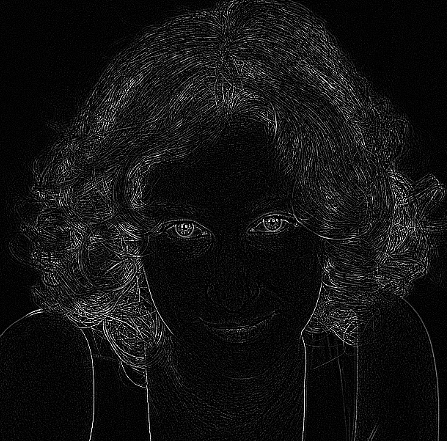
\includegraphics[width=\linewidth]{lena_lapl}}
%  \vspace{1.5cm}
  \centerline{(b) Laplaciano de $U$.}
\end{minipage}
\hfill
\begin{minipage}{0.25\textwidth}
  \centering
  \centerline{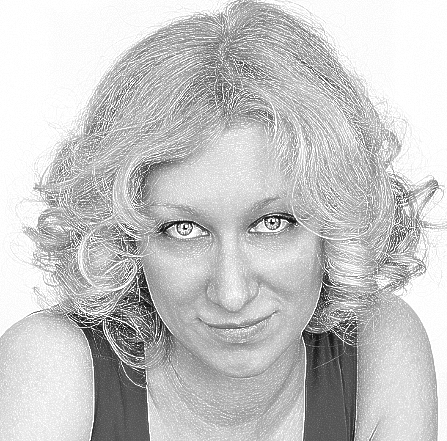
\includegraphics[width=\linewidth]{lena_sharp}}
%  \vspace{1.5cm}
  \centerline{(c) Imagen de salida $U_{\textrm{USM}}$.}\medskip
\end{minipage}
%
\caption[Ejemplo de mejora en imagen con \engl{Unsharp Mask}]{Salida del filtro USM con $\lambda = 5$ y $\sigma = 0.01$. \label{fig:exampleUSM}}
%
\end{figure}


\section{Filtro Deceived Non-Local Means}
\label{ch:marco_dnlm}


El enfoque del filtro \engl{Deceived Non-Local Means} (DNLM) consiste en la combinación de un método de \engl{Unsharp Masking} (USM) con el filtro NLM, con el propósito de lograr por un lado una mejora en los bordes y en el contraste de la imagen, y por otro lado la eliminación del ruido gausiano  presente en la imagen. La combinación propuesta se basa en el desacople entre la imagen usada en el pesado (imagen original $U$) y la utilizada en el filtrado $U_{\textrm{USM}}$. Esto permite evitar el efecto anillo presente en las im\'agenes filtradas con el USM \cite{calderon2015dewaff}.

La función del filtro DNLM est\'a dada por:

\begin{equation}
\label{eq:dnlm}
Y(U,p)=\left(\sum_{m\in \Omega}\psi_{NLM}\left(U, p, m\right)\right)^{-1} \\ \left(\sum_{m\in \Omega}\psi_{\textrm{NLM}}\left(U, p, m\right)U_{\textrm{USM}}(m)\right) \enspace ,
\end{equation}

donde $U$ es la imagen de entrada, $p$ es el pixel que se pretende filtrar, $m$ corresponde a un pixel contenido en la ventana deslizante $\Omega$, $\psi_{\textrm{NLM}}$ es una función de pesado del filtro NLM y $U_{\textrm{USM}}$ la imagen producto de la mejora con el método USM \cite{calderon2015dewaff}. El desacople mostrado en (\ref{eq:dnlm}) se da al realizar el c\'alculo de los pesos con la imagen de entrada $U$ y el filtrado con la imagen $U_{\textrm{USM}}$.

La figura \ref{fig:exampleDNLM} muestra el aumento en contraste de la imagen y el mayor detalle en bordes resultado del procesamiento con el filtro DNLM.

\begin{figure}[H]
\centering
\begin{minipage}[b]{0.3\textwidth}
  \centering
  \centerline{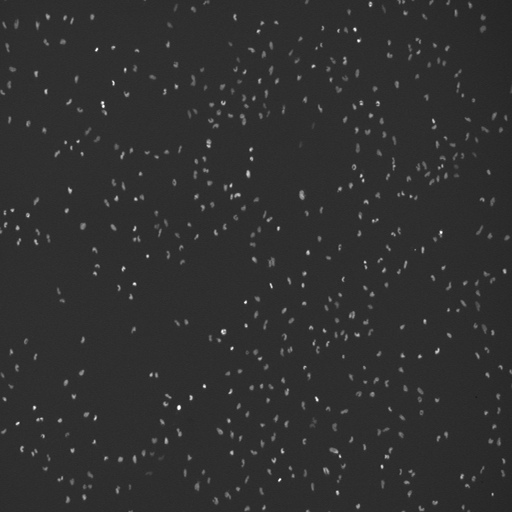
\includegraphics[width=\linewidth]{512x512}}
%  \vspace{1.5cm}
  \centerline{(a) Ejemplo de imagen de actividad celular.}\medskip
\end{minipage}
\hfill
\begin{minipage}[b]{0.3\textwidth}
  \centering
  \centerline{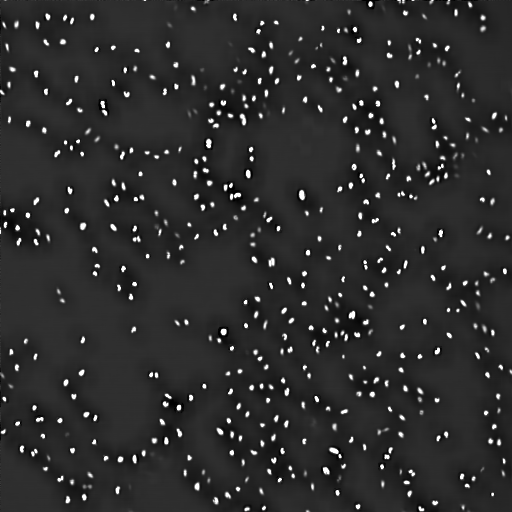
\includegraphics[width=\linewidth]{512x512_DeNLM}}
%  \vspace{1.5cm}
  \centerline{(b) Imagen fitrada.}
\end{minipage}
\vfill
\begin{minipage}[b]{0.3\textwidth}
  \centering
  \centerline{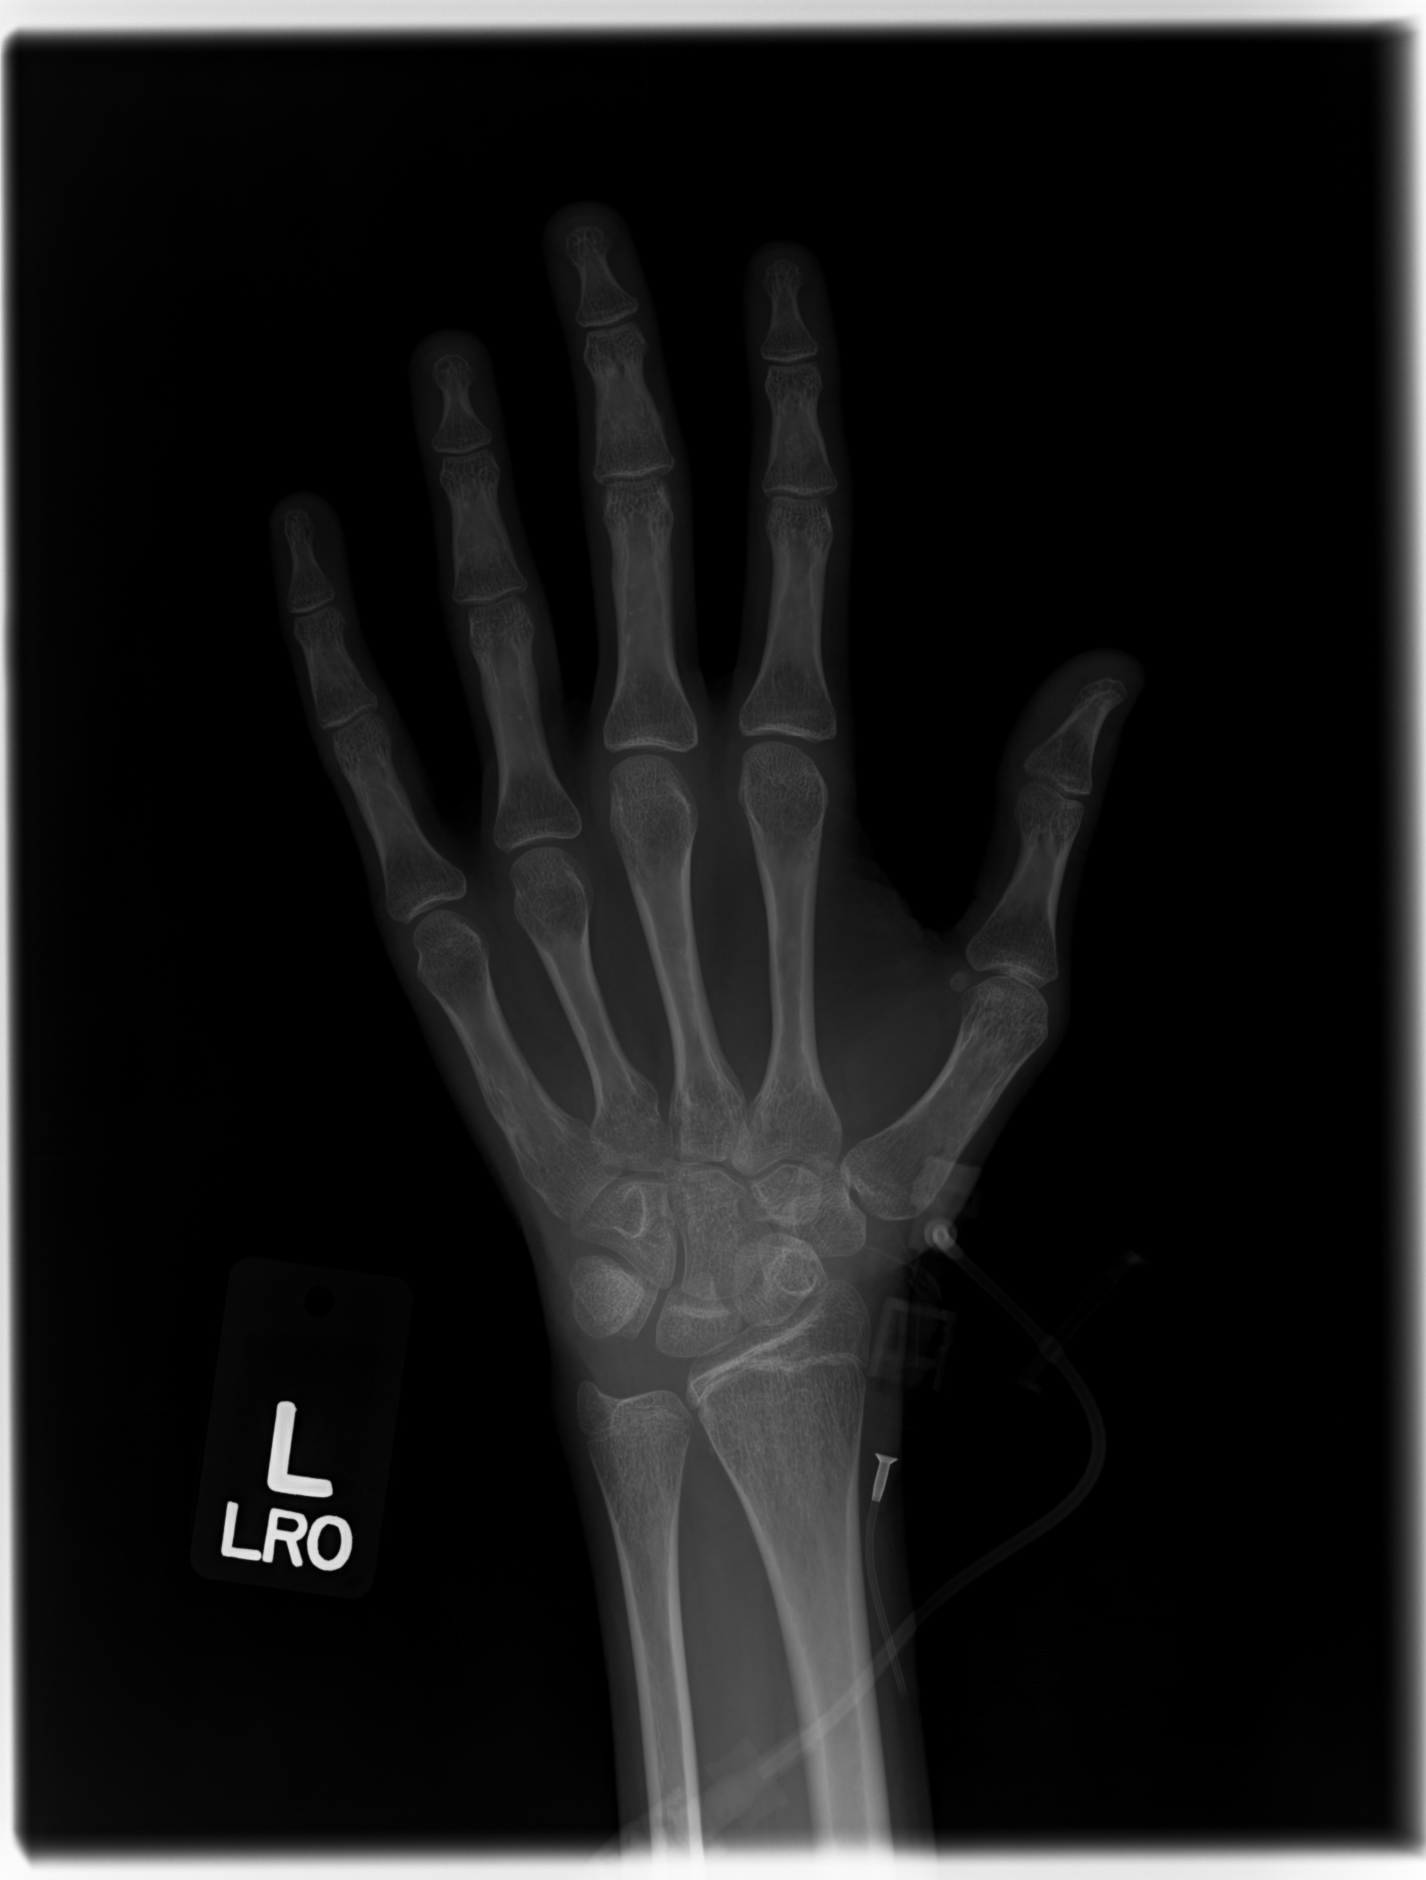
\includegraphics[width=\linewidth]{11043}}
%  \vspace{1.5cm}
  \centerline{(c) Imagen de rayos-x.}\medskip
\end{minipage}
\hfill
\begin{minipage}[b]{0.3\textwidth}
  \centering
  \centerline{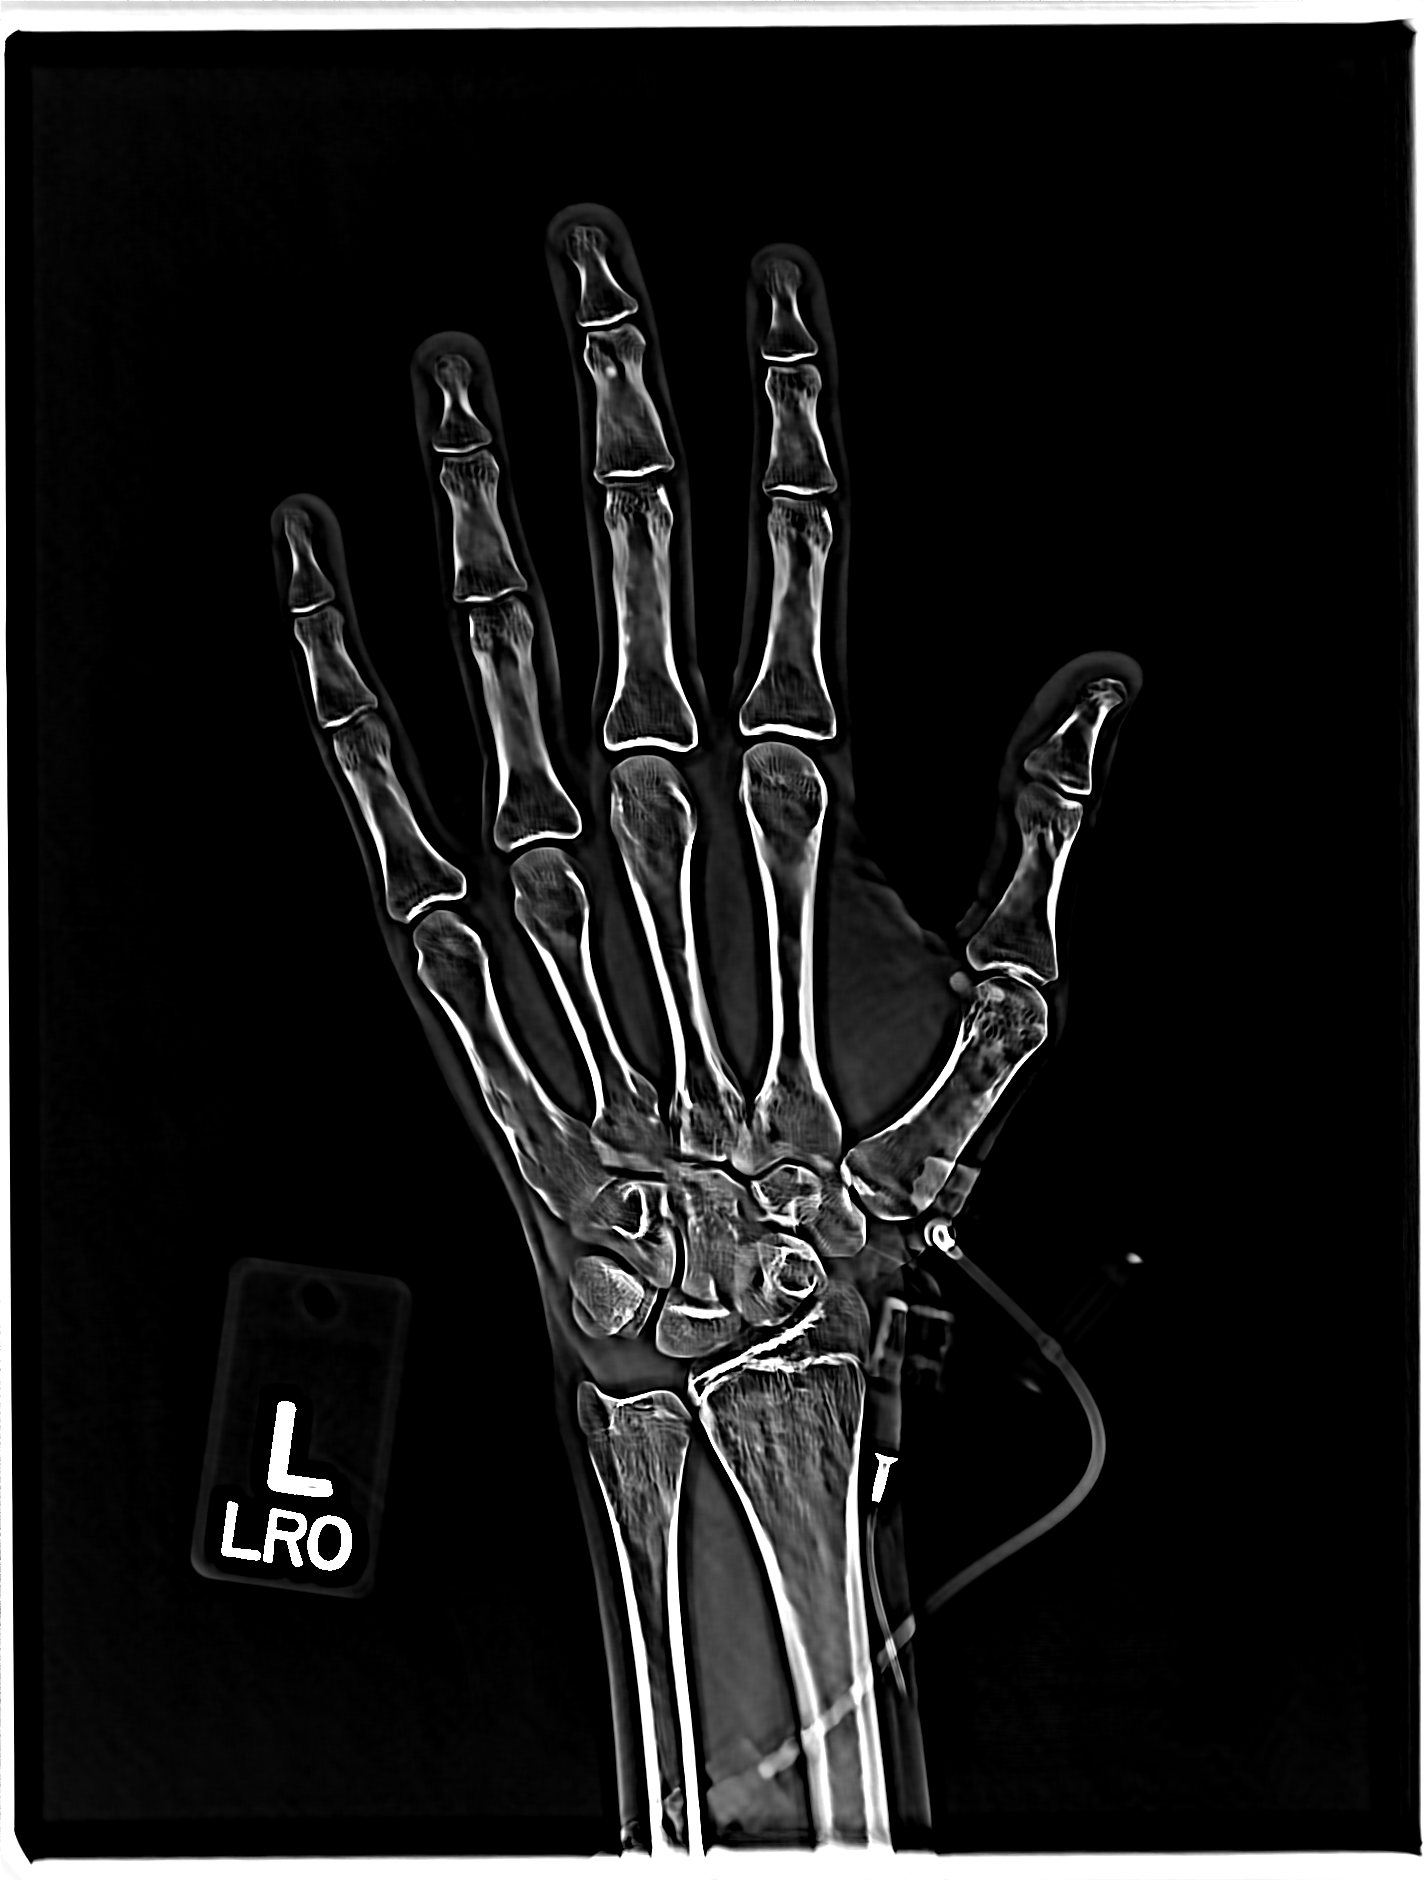
\includegraphics[width=\linewidth]{11043_DeNLM}}
%  \vspace{1.5cm}
  \centerline{(d) Imagen filtrada.}\medskip
\end{minipage}
%
\caption[Ejemplo de im\'agenes filtradas con el filtro DNLM]{Ejemplo de im\'agenes filtradas con el filtro DNLM. \label{fig:exampleDNLM}}

%
\end{figure}



\section{Optimizaciones computacionales}
\label{ch:marco_opt}

\subsection{DNLM-IIFFT}
\label{ch:marco_dnlmifft}

Esta optimización computacional utiliza im\'agenes integrales y la transformada r\'apida de Fourier para disminuir la complejidad computacional del filtro DNLM. 



Al analizar la distancia euclidiana $D$ entre los vecindarios se tiene que:

\begin{equation}
D\left(x,y\right)=\left\Vert \vec{\boldsymbol{\eta}}\left(y\right)-\vec{\boldsymbol{\eta}}\left(x\right)\right\Vert^2 \enspace . 
\end{equation}

La ecuación anterior puede representarse en notacion matricial con la norma de Frobenius $\Vert \cdot \Vert_{F}$ como:


\begin{equation}
D\left(x,y\right)=\Vert \mat{Y} - \mat{X} \Vert_{F}^2 \enspace ,
\label{eq:distMat}
\end{equation}

con \mat{Y} y \mat{X} las matrices de los vecindarios de los pixeles $y$ y $x$. respectivamente.

Si se se define la norma $\Vert \cdot \Vert_{F}^2$ con el producto interno de Frobenius $\langle\,,\rangle_{F}$ se tiene que:

\begin{equation}\label{eq:frobProd}
\begin{split}
\Vert \mat{Y} - \mat{X} \Vert_{F}^2 & = \langle\mat{Y} - \mat{X},\mat{Y} - \mat{X}\rangle_{F}  \quad \text{y por sesquilinealidad:}\\ 
& = \langle\mat{Y},\mat{Y}\rangle_{F} + \langle\mat{Y},-\mat{X}\rangle_{F} + \langle-\mat{X},\mat{Y}\rangle_{F} + \langle-\mat{X},-\mat{X}\rangle_{F}\\
& = \Vert \mat{Y} \Vert_{F}^2 -2\langle\mat{Y},\mat{X}\rangle_{F} + \Vert \mat{X} \Vert_{F}^2 \enspace ,
\end{split} 
\end{equation}


tomando en cuenta que $\Vert \cdot \Vert_{F}^2$ es una norma que cumple todos los axiomas correspondientes. 

\begin{table}
\begin{center}
\caption{Ejemplo de imagen de entrada \mat{U}.\label{table:imageExample}}

\renewcommand{\arraystretch}{1.4}
\setlength\tabcolsep{3pt}

{
\begin{tabular}{cc|ccc|c}
 & \multicolumn{1}{c}{\textbf{1}} & \textbf{2} & \textbf{3} & \multicolumn{1}{c}{\textbf{4}} & \textbf{5}\tabularnewline
\textbf{1} & \multicolumn{1}{c}{5} & 12 & 1 & \multicolumn{1}{c}{3} & 2\tabularnewline
\cline{3-5} 
\textbf{2} & 5 & 2 & 3 & 1 & 4\tabularnewline
\textbf{3} & 3 & 1 & \textbf{2} & 3 & 1\tabularnewline
\textbf{4} & 4 & 3 & 2 & 1 & 3\tabularnewline
\cline{3-5} 
\textbf{5} & \multicolumn{1}{c}{1} & 5 & 6 & \multicolumn{1}{c}{5} & 3\tabularnewline
\end{tabular}
}
\par\end{center} 
\end{table}

El siguiente ejemplo ilustra el cálculo de la norma de Frobenius entre los vecindarios de pixeles contenidos en la imagen $\mat{U} \in\mathbb{R}^{5 \times 5}$ definida en la Tabla \ref{table:imageExample}. Para efectos de la ilustración, se toman los vecindarios $\mat{P}_{\left(3,3\right)},\mat{P}_{\left(2,2\right)} \in\mathbb{R}^{3\times3}$ de la imagen de ejemplo \mat{U}  y se realiza  el cálculo de la norma de Frobenius tal que:


\begin{equation}
\label{eq:resultado1}
\begin{split}
\left\Vert \mat{P}_{\left(3,3\right)}-\mat{P}_{\left(2,2\right)}\right\Vert_{F} ^{2} & =\left\Vert \left[\begin{array}{ccc}
2 & 3 & 1\\
1 & 2 & 3\\
3 & 2 & 1
\end{array} \right]-\left[\begin{array}{ccc}
5 & 12 & 1\\
5 & 2 & 3\\
3 & 1 & 2
\end{array}\right]\right\Vert_{F}^2 \\
& =\left\Vert\left[\begin{array}{ccc}
-3 & -9 & 0\\
-4 & 0 & 0\\
0 & 1 & -1
\end{array}\right]\right\Vert_{F}^2 \\
& =108 \enspace .
\end{split}
\end{equation}



Al desarrollar (\ref{eq:resultado1}) como se muestra en (\ref{eq:frobProd}), se obtiene que: 
\begin{equation}\label{eq:matFrodProd}
\resizebox{.9 \textwidth}{!} 
{
$\begin{split}
\lVert \mat{P}_{\left(3,3\right)}-\mat{P}_{\left(2,2\right)}\rVert_{F} ^{2} & =\lVert \mat{P}_{\left(3,3\right)}\rVert_{F}^2 -2\langle\mat{P}_{\left(3,3\right)},\mat{P}_{\left(2,2\right)}\rangle_{F} + \lVert \mat{P}_{\left(2,2\right)}\rVert_{F}^2  \\
& = \left\Vert\left[\begin{array}{ccc}
2 & 3 & 1\\
1 & 2 & 3\\
3 & 2 & 1
\end{array}\right]\right\Vert_{F}^2-2\left\langle\left[\begin{array}{ccc}
2 & 3 & 1\\
1 & 2 & 3\\
3 & 2 & 1
\end{array}\right],\left[\begin{array}{ccc}
5 & 12 & 1\\
5 & 2 & 3\\
3 & 1 & 2
\end{array}\right]\right\rangle_{F}
+\left\Vert\left[\begin{array}{ccc}
5 & 12 & 1\\
5 & 2 & 3\\
3 & 1 & 2
\end{array}\right]\right\Vert_{F}^2 \\
& =42+-2\cdot78+222\\
& =42-156+222\\
& =108 \enspace ,
\end{split}$
}
\end{equation}


consistente con los resultados obtenidos en (\ref{eq:resultado1}).




Esta optimización del filtro DNLM se centra en el cálculo de la norma de Frobenius desarrollada en  (\ref{eq:frobProd}) de la siguiente manera:

\begin{itemize}
\item El uso de la imagen integral cuadrática para calcular los términos $\Vert \mat{Y} \Vert_{F}^2 $ y $\Vert \mat{X} \Vert_{F}^2 $.
\item Calcular la convolución para obtener el término $-2\langle\mat{Y},\mat{X}\rangle_{F} $
correspondiente a la correlación del vecindario \mat{Y} con la ventana de búsqueda \mat{\Omega}, para acceder posteriormente al $i$-ésimo elemento del resultado.
\end{itemize}

Lo anterior permite disminuir la complejidad computacional del filtro a $O(S\log(S) \cdot N)$.
 
\subsubsection{Imágenes integrales}


La imagen integral $\mat{I}_{\Sigma}$ de una imagen de entrada \mat{U} presentada en \cite{viola2001robust}, está dada por: 
\begin{equation}
\mat{I}_{\Sigma}\left(x,y\right)=\sum_{i\leq x}\sum_{j\leq y}u_{ij} \enspace ,
\end{equation}
la cual corresponde a la sumatoria de todos los  pixeles ubicados a la izquierda y superiores al pixel $u_{ij}$ de la imagen de entrada \mat{U}.

\begin{table}
\begin{center}
\caption{Ejemplo de imagen de entrada \mat{U^{\odot 2}}.\label{table:imageExample2}}

\renewcommand{\arraystretch}{1.4}
\setlength\tabcolsep{3pt}

{
\begin{tabular}{cc|ccc|c}
 & \multicolumn{1}{c}{\textbf{1}} & \textbf{2} & \textbf{3} & \multicolumn{1}{c}{\textbf{4}} & \textbf{5}\tabularnewline
\textbf{1} & \multicolumn{1}{c}{5} & 12 & 1 & \multicolumn{1}{c}{3} & 2\tabularnewline
\cline{3-5} 
\textbf{2} & 25 & 4 & 9 & 1 & 16\tabularnewline
\textbf{3} & 9 & 1 & \textbf{2} & 9 & 1\tabularnewline
\textbf{4} & 16 & 9 & 4 & 1 & 9\tabularnewline
\cline{3-5} 
\textbf{5} & \multicolumn{1}{c}{1} & 5 & 6 & \multicolumn{1}{c}{5} & 3\tabularnewline
\end{tabular}
}
\par\end{center} 
\end{table}


Continuando con el ejemplo previamente mostrado, la imagen de entrada \mat{U} con sus elementos elevados al cuadrado se define como el producto de Hadamard $\mat{U}^{\odot 2} = \mat{U} \odot \mat{U}$, como se muestra en la tabla \ref{table:imageExample2}. 


\begin{table}
\caption{Imagen integral para $U^{\odot2}$.\label{table:integralcuad}}
\begin{center}
\renewcommand{\arraystretch}{1.4}
\setlength\tabcolsep{3pt}
{
\begin{tabular}{cc|ccc|c}
 & \multicolumn{1}{c}{\textbf{1}} & \textbf{2} & \textbf{3} & \multicolumn{1}{c}{\textbf{4}} & \textbf{5}\tabularnewline
\textbf{1} & \multicolumn{1}{c}{\textbf{25(a)}} & 169 & 170 & \multicolumn{1}{c}{\textbf{179(b)}} & 183\tabularnewline
\cline{3-5} 
\textbf{2} & 50 & 198 & 208 & 218 & 238\tabularnewline
\textbf{3} & 59 & 208 & \textbf{222} & 241 & 262\tabularnewline
\textbf{4} & \textbf{75(c)} & 233 & 251 & \textbf{271(d)} & 301\tabularnewline
\cline{3-5} 
\textbf{5} & \multicolumn{1}{c}{76} & 259 & 313 & \multicolumn{1}{c}{358} & 397\tabularnewline
\end{tabular}
}
\par\end{center}
\end{table}


La imagen integral $\mat{I}_{\Sigma}$ se puede calcular iterativamente para un pixel específico de la imagen de entrada \mat{U} de la siguiente manera: 
\begin{equation}
\mat{I}_{\Sigma}\left(x,y\right)=\mat{U}\left(x,y\right)-\mat{I}_{\Sigma}\left(x-1,y-1\right)+\mat{I}_{\Sigma}\left(x,y-1\right)
+\mat{I}_{\Sigma}\left(x-1,y\right) \enspace ,
\end{equation}

lo cual, para el ejemplo anterior significa que:

\begin{equation}
\mat{I}_{\Sigma}\left(3,3\right)=4-198+208+208=222 \enspace .
\end{equation}

Las imágenes integrales son útiles para calcular la sumatoria sobre una región determinada de la imagen, con una complejidad computacional constante de $\mathcal{O}(1)$. 

Al utilizar la imagen integral $\mat{I}_{\Sigma}$ para calcular la sumatoria de una región de la imagen original \mat{U}, limitada por los pixeles $a=\left(x_{0},y_{0}\right)$,
$b=\left(x_{1},y_{0}\right)$, $c=\left(x_{0},y_{1}\right)$ and $d=\left(x_{1},y_{1}\right)$, ilustrados en la Tabla \ref{table:integralcuad}, se calcula como: 

\begin{equation}
\sum_{i>x_{0}}^{i\leq x_{1}}~\sum_{j>y_{0}}^{j\leq y_{1}}u_{ij}=\mat{I}_{\Sigma}\left(d\right)+\mat{I}_{\Sigma}\left(a\right)-\mat{I}_{\Sigma}\left(b\right)-\mat{I}_{\Sigma}\left(c\right) \enspace ,
\end{equation}

y en el ejemplo presentado para una ventana de $3\times3$ pixeles alrededor del pixel $u_{3,3}^2$ de la imagen $\mat{U}^{\odot2}$ , los pixeles de las esquinas están dados por: $a=\left(1,1\right)$, $b=\left(4,1\right)$,
$c=\left(1,4\right)$ y $d=\left(4,4\right)$, como se muestra en la Tabla \ref{table:imageExample2}. El cálculo de la sumatoria de los pixeles en la región especificada está dada por: 

\begin{equation}
\sum_{i>1}^{i\leq 4}~\sum_{j>1}^{j\leq 4}u_{i,j}^2=271+25-179-75=42 \enspace ,
\end{equation}

lo cual, es consistente con el término $\mat{P}_{\left(3,3\right)}$ en (\ref{eq:matFrodProd}). 



\subsubsection{Convolución y transformada rápida de Fourier}

Como se mostró anteriormente, el término $-2\langle\mat{Y},\mat{X}\rangle_{F}$ producto del desarrollo de la norma de Frobenius en (\ref{eq:matFrodProd}), puede representarse como el $i$-ésimo elemento de la matriz resultante de la correlación del vecindario \mat{X} del pixel $x_{ij}$ con la ventana \mat{\Omega} como:

\begin{equation}
-2\langle\mat{Y},\mat{X}\rangle_{F} = -2\left[\mat{\Omega} \otimes \mat{X}\right](i,j) \enspace .
\end{equation}

Para expresar la correlación en términos de la convolución, se debe rotar la matriz \mat{X} de modo que se cumple que:

\begin{equation}
\mat{\Omega} \otimes \mat{X} = \mat{\Omega}*\mat{X}\mat{I}^T \enspace ,
\end{equation}

donde $\mat{I}^T$ es la matriz identidad transpuesta del vecindario \mat{X}. Lo anterior implica que el término sea calculado como:

\begin{equation}
-2\langle\mat{Y},\mat{X}\rangle_{F} = -2\left[\mat{\Omega} *\mat{X}\mat{I}^T\right](i,j) \enspace .
\end{equation}




\subsection{DNLM-MA}
\label{ch:marco_condat}

Esta propuesta de optimización computacional del filro NLM se caracteriza por su simpleza, al proponer un intercambio entre los ciclos de interación del algoritmo \cite{Condat2010}. La aceleración se consigue al incorporar simetría y convoluciones al realizar el ponderamiento de la regón definida por la ventana de búsqueda \mat{\Omega}, para todos los pixeles la imagen de manera simultánea.

Siguiendo la definición de la función de pesado del filtro NLM en (\ref{eq:nlmfunc}), un pixel $y$ puede ser expresado en términos del desplazamiento desde un pixel $x$ como $y = x + \Delta$. Por ejemplo, para una ventana de búsqueda $\vert\Omega\vert = 5 \times 5$, $\Delta$ puede tomar los valores $\Delta=0$, $\Delta=1$, $\Delta=2$ y en general, puede tomar valores de hasta $\Delta=\vert\Omega\vert/2$. Por lo tanto, la función de pesado del filtro NLM es simétrica si:

\begin{equation}\
\psi_{\text{NLM}}(\mat{U}, x, x + \Delta) = \psi_{\text{NLM}}(\mat{U}, y, y - \Delta)  \enspace . 
\label{eq:symmetry}
\end{equation}

Los pesos son calculados al intercambiar los ciclos del algoritmo, ya que se itera sobre cada desplazamiento $\Delta$, en lugar de iterar sobre cada uno de los pixeles de la imagen de entrada. Para cada una de las iteraciones, la diferencia cuadrática es calculada para toda la imagen como:

\begin{equation}
\mat{D}_\Delta\left(x\right) = \left(\mat{U}\left(x\right) - \mat{U}\left( x + \Delta \right)\right)^{\circ2}  \enspace ,
\label{eq:diffquad}
\end{equation}

donde la potencia al cuadrado es para cada pixel individual, siguiendo la notación de Hadamard. Seguidamente, se calcula la convolución de
$\mat{D}_\Delta$ con un kernel de promediado de tama\~no $\omega$ de la siguiente forma:
\begin{equation}
\label{eq:convmoas}
\mat{E}_{\Delta} = \mat{D}_{\Delta} * \mat{G} \enspace ,
\end{equation}

donde se define la convolución con un kernel $h$ (\ref{eq:convmoas}) que corresponde a un kernel de promediado.


El resultado es la función de pesado del filtro DNLM-MA: 

\begin{equation}
\psi_{DNLM-MA}=\exp^{\circ}\left(-\frac{ E_\Delta\left(x\right) }{h}\right)  \enspace .
\label{eq:wmoas}
\end{equation}


Con esto se consigue reducir la  función de costo computacional a $O(\sqrt{P} \cdot S \cdot N)$.  



\section{Arquitectura Intel Xeon Phi Knights Landing}
\label{ch:marco_xeonphi}

La arquitectura de procesador Intel Xeon Phi Knights Landing conocida como \textit{many-core} está dise\~nada para aplicaciones de computación de alto rendimiento y es considerada la alternativa de Intel al desarrollo de algoritmos en GPU para propósito general. A diferencia de la versión anterior, esta nueva iteración con nombre clave Knights Landig permite el arranque de un sistema operativo por sí misma y provee más de 3 TFLOP/s de precisión doble y cerca de 6 TFLOP/s de precisión doble \cite{Jeffers201663}. Posee de 32 a 36 celdas interconectadas por una interfaz de comunicación en 2D, cada una de ellas conformada por 2 CPU y 1MB de caché L2 compartido \cite{XeonPhiWhitePaper}. Cada uno de los CPU incorpora 2 Unidades de Procesamiento Vectorial (VPU) con registros de hasta 512 bytes de largo, capaces de operar de manera simultánea para 2 o más hilos \ref{XeonPhiWhitePaper}. 
Entre las características que destacan del CPU es su modo de ejecución fuera de orden y el multihilo simultáneo de 4 hilos \cite{XeonPhiWhitePaper}. Una de sus particularidades es la incorporación de 16GB de Memoria de Alto Ancho de Banda (MCDRAM) de hasta $450 Gbyte/s$ en el mismo chip como lo muestra la Figura \ref{fig:cpu_phi}, permitiendo tiempos de latencia cortos en comparación con los obtenidos con tecnologías DDR4 \cite{XeonPhiWhitePaper}.

\begin{figure}
\centering
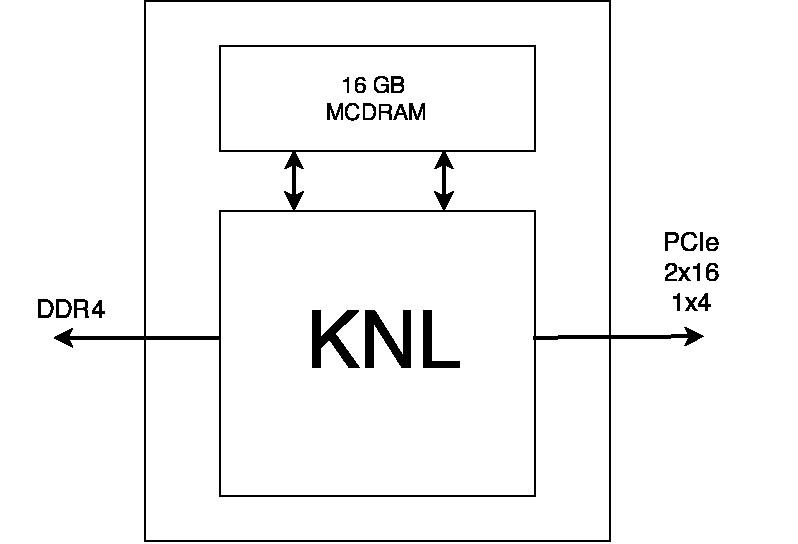
\includegraphics[width=0.5\textwidth]{fig/cpu}
\caption{Diagrama de alto nivel del procesador Xeon Phi KNL.}
\label{fig:cpu_phi}
\end{figure}


La arquitectura KNL presenta distintos modos de configuración de memoria y \engl{clústering}. Para efectos de este trabajo, se utiliza el modo de configuración recomendado por el fabricante: Modo de \engl{clustering} por cuadrantes y configuración de memoria MCDRAM como \engl{caché}.


\section{Paralelización y vectorización}
\label{ch:marco_parallel}

Existen múltiples enfoques de paralelización y vectorización del filtro NLM en el estado del arte. Estos han demostrado una alta aceleración del algoritmo de filtrado, como lo muestra la Tabla \ref{method_table}. 


\begin{table}
\caption[Estado del arte en paralelizaciones del filtro NLM]{Métodos previos de implementaciones paralelas para el filtro NLM. Se muestra únicamente la aceleración máxima respecto a la versión secuencial no optimizada del filtro.}
\begin{tabularx}{1\linewidth}{X X X X} 
\hline
Implementación & Arquitectura & Método & Aceleración \\ [0.5ex]
 \hline\hline
 Coupe et al. \cite{coupe2006fast} &  8 Intel Xeon CPU & Biblioteca de Hilos & $50\times$\\
 Darbon et al. \cite{Darbon2008} &  8 Dual-Core AMD Opteron CPU & Instrucciones Vectorizadas & $110\times$\\
 Mingliang et al. \cite{mingliang2016medical} &  NVIDIA Quadro FX 480 & CUDA & $40\times$\\
Gossens et al. \cite{goossens2010gpu} &  NVIDIA GeForce 9600 GT & DirectX & $402\times$\\
Marques and Pardo. \cite{marques2013implementation} &  NVIDIA GeForce GTX 680 & CUDA & $718\times$\\ 
Shi et al. \cite{shi2015optimized} &   1024 núcleos SuperMUC & MPI & $740\times$\\
Nguyen et al. \cite{nguyen2016medical} &   8 Intel Xeon CPU & MPI y PThreads & $148\times$\\
Nguyen et al. \cite{nguyen2016medical} &   8 NVIDIA Tesla C2050 & MPI y CUDA & $510\times$\\
Zhu et al. \cite{zhu2016parallel} &  Intel Xeon Phi 7110P & OpenMP & $87\times$\\
Zhu et al. \cite{zhu2016parallel} &  Intel Xeon Phi 7110P & OpenCL & $108\times$\\
Huang et al. \cite{huang2017parallel} &  Intel Xeon Phi & OpenMP & $32\times$\\
\end{tabularx}
\label{method_table}
\end{table}

La primera implementación paralela encontrada en la literatura se realiz\' mediante múltiplles hilos de ejecución para procesar imágenes médicas en 3D, con la ayuda de un servidor y 8 procesadores Xeon \ \cite{coupe2006fast}. Seguidamente, se utiliza una arquitectura SIMD para paralelizar el filtro en un servidor con 8 procesadores AMD Opteron de doble núcleo \cite{Darbon2008}. Además, implementaciones en GPU han empleado la optimización propuesta por Gossens en DirectX \cite{marques2013implementation} y la optimización propuesta por Condat en CUDA \cite{mingliang2016medical,goossens2010gpu}, las cuales muestran mayores aceleraciones que las implementaciones en CPU. Otra implementación con una aceleración ligeramente mayor a la obtenida por Marques y Pardo \cite{marques2013implementation} es conseguida en un sistema distribuido con 1024 núcleos de procesamiento \cite{shi2015optimized}. Una implementación más compleja combina MPI con P-Threads y MPI con CUDA para alcanzar una aceleración aún mayor \cite{nguyen2016medical}. Finalmente, dos implementaciones del filtro para plataformas Xeon Phi \cite{zhu2016parallel,huang2017parallel} y OpenCL \cite{zhu2016parallel}.

Si bien la aceleración obtenida con GPU es usualmente mayor a las reportadas con la plataforma Xeon Phi, ésta última tiene la ventaja de proveer un estilo de programación sencillo y flexible, ya que utiliza el set de instrucciones X86 \cite{huang2017parallel}. 

La arquitectura KNL está dise\~nada con un fuerte soporte de instrucciones vectoriales para acelerar operaciones sobre datos, sin embargo,  la vectorización se ve afectada si no se asegura un correcto alineamiento de los datos, o bien si el pre-retiro de instrucciones de caché no es efectivo \cite{Jeffers201617:vect}.
La vectorización de las rutinas del algoritmo son fundamentales para acelerar el tiempo de procesamiento en la arquitectura KNL. Por ejemplo, utilizar instrucciones vectoriales como AVX-512 permite el cálculo simultaneo de 16 operaciones matemáticas de precisión simple, o bien 8 operaciones de precisión doble \cite{Jeffers201617:vect}.

Una efectiva vectorización se puede lograr con tres enfoques:

\begin{itemize}
\item Bibliotecas: Muchas bibliotecas se encuentran previamente optimizadas para el uso de instrucciones vectorizadas. 
\item Auto-vectorización: Consiste en otorgarle la responsabilidad al compilador para identificar regiones vectorizables.
\item Directivas o \engl{pragmas} para assistir vectorización: Permite que el programador le indique al compilador las regiones paralelizables.
\end{itemize}
 
En este trabajo se apuesta por la primera opción: el uso de la biblioteca \engl{Intel Performance Primitives} (IPP). Esta biblioteca incorpora rutinas vectorizadas con datos alineados en memoria para funciones de procesamiento de se\~nales e imágenes. Además, la biblioteca IPP implementa un despachador que selecciona atomáticamente el conjunto de instruccions SIMD específico para las rutinas de la biblioteca, de acuerdo a las características del procesador \cite{IntelCorporation2017}.  Sumado a lo anterior, permite selccionar un conjunto de instrucciones SIMD específico \cite{IntelCorporation2017}, siendo útil para comprobar la diferencia en rendimiento entre diferentes conjuntos de instrucciones SIMD según se requiera.

El filtro DNLM tiene la ventaja de poder realizar el filtrado de cada pixel de manera independiente. Esto se puede intuir de la función de filtrado (\ref{eq:weighted}). El resultado tiene un alto nivel de paralelismo, con un grado de granularidad propicio para distribuir la carga de procesamiento en los núcleos del procesador, como se observa en la Figura \ref{fig:parallel_figure}. 



\begin{figure}[H]
   \centering
   \caption[Diagrama de distribución de tareas paralelas]{Diagrama de distribución de tareas para la paralelización del filtro DNLM}
   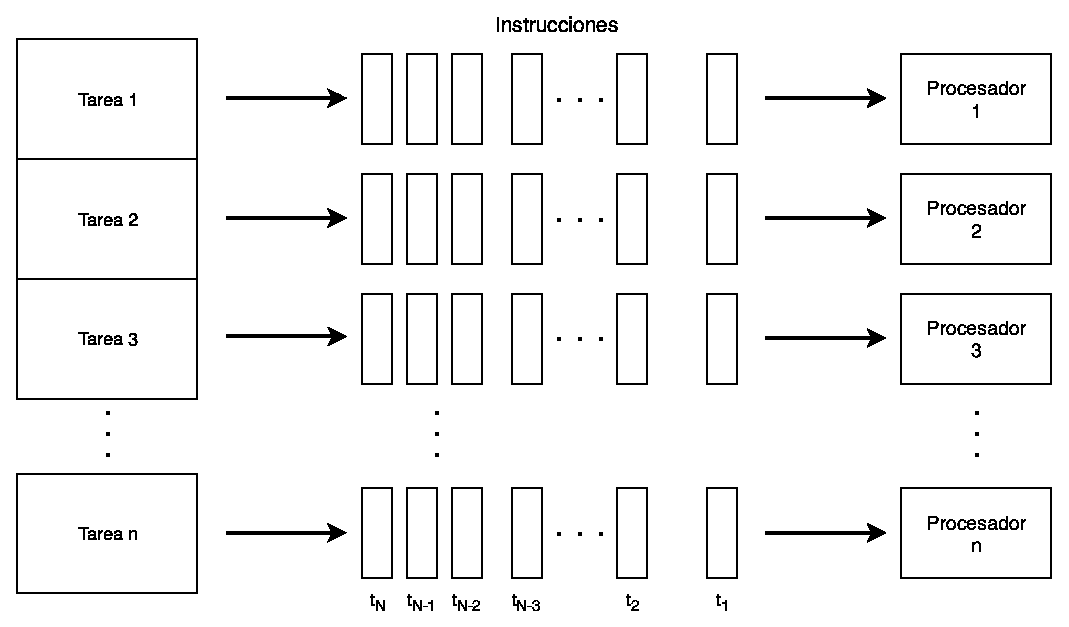
\includegraphics[width=0.8\textwidth]{parallel_figure}
   \label{fig:parallel_figure}
 \end{figure}
 
 
 Los ciclos son regiones de código potencialmente paralelizables, con excepción de aquellos donde exista dependencia entre iteraciones. 
 
\subsubsection{Métricas para evaluar paralelización y vectorización}
 
Existen métricas para evaluar el comportaminto de los algoritmos y se obtienen por medio de la lectura de registros especializados en el KNL. Estas métricas se pueden obtener gracias al muestreo de estos registros por medio de las herramientas de perfilado. Dichas métricas son útiles para identificar las secciones del programa donde las optimizaciones pueden generar un impacto en el tiempo de ejecución.

El proceso de ajuste del rendimiento del algoritmo pasa por conocer cómo se ejecutan las aplicaciones a nivel de los componentes en la arquitectura como \engl{pipelines}, cachés, VPU, etc.

Las métricas utilizadas en este trabajo se listan a continuación:

\paragraph*{Ciclos por instrucción (CPI):}

Esta métrica consiste en el número promedio de ciclos requeridos por hilo para ejecutar una instrucción y se considera como un indicador de la latencia presente, que afecta el tiempo de ejecución de una aplicación.

La métrica CPI promedio por hilo está dada por:
\begin{equation}\label{eq:CPI_metric}
\text{CPI}_{\text{hilo}} = \frac{\text{\# de ticks de reloj}}{\# \text{de instrucciones}}
\end{equation}

Además, se puede calcular los CPI promedio por CPU como:

\begin{equation}\label{eq:CPIc_metric}
\text{CPI}_{\text{CPU}} = \frac{\text{CPI}_{\text{hilo}}}{\text{cantidad CPU}}
\end{equation}

El valor de $\text{CPI}_{\text{CPU}} $ se reduce al aumentar la cantidad de hilos de ejecución, por lo tanto, al optimizar se debe conseguir el menor $\text{CPI}_{\text{CPU}} $. Además, se debe tomar en cuenta que al utilizar instrucciones vectoriales el CPI tiende a aumentar, debido a que la cantidad de trabajo realizado con una sóla instrucción aumenta \cite{Jeffers2016315}.

\paragraph*{Uso de VPU}

Esta métrica permite obtener la intensidad en instrucciones vectorizables a razón de las instrucciones escalares, dando una medida de la eficiencia en términos de opraciones en punto flotante por segundo\cite{Jeffers2016315}. Esá definida como:

\begin{equation}
\text{VPUi}= \frac{\text{\# SIMD empaquetadas}}{\text{\# SIMD empaquetadas}+\text{\# SIMD escalares}}
\end{equation}
